\section{Experiments}
\label{sec:experiments}

In this chapter, we will describe the experiments which were used to evaluate online scheduling systems. Each experiment was run for each online scheduling algorithm. Also, each experiment was repeated $10$ times, to be able to draw statistically significant conclusions.

The idea behind these experiments was to create a simple but diverse set of case studies with different behaviors and event types.

\subsection{Experiment 1}

The topology for the first experiment is shown in figure \ref{fig:experiment1_topology}. In this experiment, machines would occasionally have breakdowns. There were two types of jobs. Jobs of the first type generally had lower weights, but they could be preempted, while jobs of the second type generally had higher weights, but they could not be preempted. In the train job sequence, there were a total of $200$ jobs, $100$ of each type. In the test job sequence, there were a total of $600$ jobs, $300$ of each type.

\begin{figure}[!htbp]
	\centering
	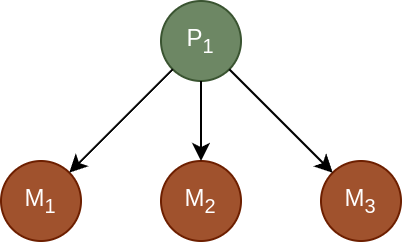
\includegraphics[scale=0.6]{../images/experiment1_topology.png}
	\caption{Experiment 1 - topology}
    \label{fig:experiment1_topology}
\end{figure}

\subsection{Experiment 2}

The topology for the second experiment is shown in figure \ref{fig:experiment2_topology}. In this experiment, there were three job types, and preemptions were allowed for all of them. The batch processing limit of every job type on the machines was $3$. In the train job sequence, there were a total of $240$ jobs, $80$ of each type. In the test job sequence, there were a total of $600$ jobs, $200$ of each type.

\begin{figure}[!htbp]
	\centering
	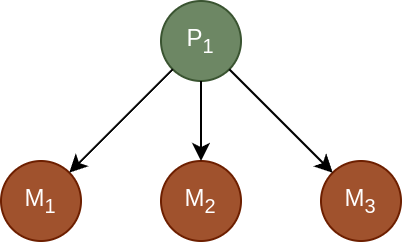
\includegraphics[scale=0.6]{../images/experiment2_topology.png}
	\caption{Experiment 2 - topology}
    \label{fig:experiment2_topology}
\end{figure}

\subsection{Experiment 3}

The topology for the third experiment is shown in figure \ref{fig:experiment3_topology}. In this experiment, every machine had a buffer of size $3$, and some jobs had prerequisites in regards to jobs which entered the system before. In each parallel group, there were two fast machines, and one which was slower in processing jobs. In the train job sequence, there were a total of $200$ jobs. In the test job sequence, there were a total of $500$ jobs.

\begin{figure}[!htbp]
	\centering
	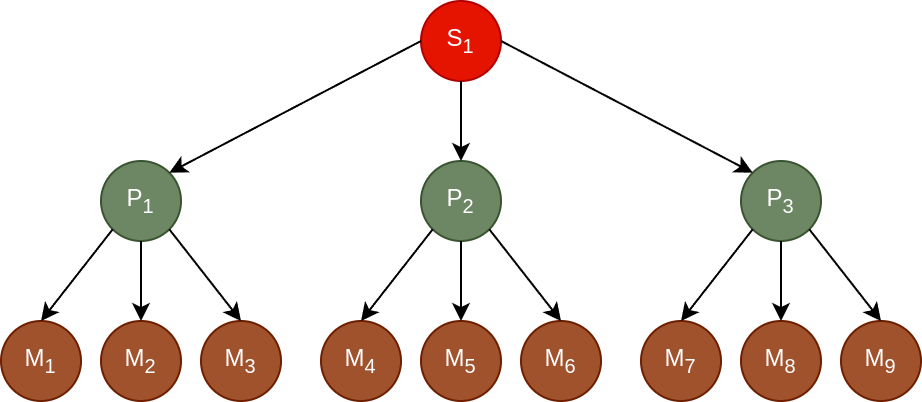
\includegraphics[scale=0.6]{../images/experiment3_topology.png}
	\caption{Experiment 3 - topology}
    \label{fig:experiment3_topology}
\end{figure}

\subsection{Experiment 4}

The topology for the fourth experiment is shown in figure \ref{fig:experiment4_topology}. In this experiment, a total of $3$ jobs could be processed in a batch. Also, there was a setup on every machine between processing two jobs, which took half the time that the processing of a job on a machine took. In the train job sequence, there were a total of $200$ jobs. In the test job sequence, there were a total of $500$ jobs.

\begin{figure}[!htbp]
	\centering
	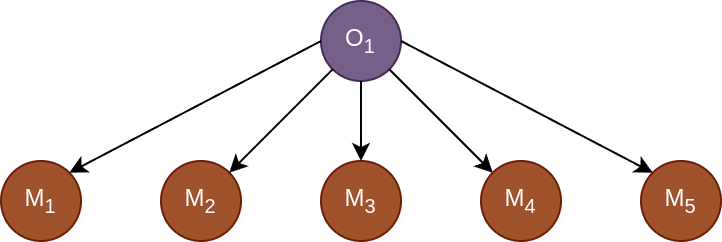
\includegraphics[scale=0.6]{../images/experiment4_topology.png}
	\caption{Experiment 4 - topology}
    \label{fig:experiment4_topology}
\end{figure}

\subsection{Experiment 5}

The topology for the fifth experiment is shown in figure \ref{fig:experiment5_topology}. In this experiment, jobs could be preempted from machines, and there was a setup on every machine between processing two jobs, which took half the time that the processing of a job on a machine took, the same as the previous experiment. In the train job sequence, there were a total of $200$ jobs. In the test job sequence, there were a total of $500$ jobs.

\begin{figure}[!htbp]
	\centering
	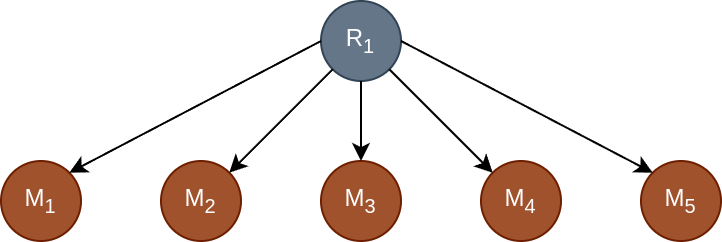
\includegraphics[scale=0.6]{../images/experiment5_topology.png}
	\caption{Experiment 5 - topology}
    \label{fig:experiment5_topology}
\end{figure}